\documentclass[12pt, a4paper,twoside]{tesi_upf}


\usepackage[applemac]{inputenc}


%IDIOMES
\usepackage[english,catalan]{babel}
\usepackage[cam,a4,center,frame]{crop}
\usepackage[colorlinks=false]{hyperref}
\usepackage{graphicx}
\usepackage{mathtools}
\usepackage{csquotes}
\usepackage{times}
%\usepackage{garamond}
\pagestyle{plain}
\usepackage[backend=biber,backref]{biblatex}
\usepackage{biblatex}
\usepackage{makeidx}
\makeindex


%\bibliographystyle{apalike}



\selectlanguage{catalan}


\addto\captionscatalan
  {\renewcommand{\contentsname}{\Large \sffamily Sumari}}
\addbibresource{../bibliography/bibliography_tesis.bib}
\addbibresource{../bibliography/library.bib}


\title{El titulo de la tesi: In-silico methods to drug discovery}
\subtitle{El subtitulo de la tesi: Cancer}
\author{Autor: Francisco Mart\'inez Jim\'enez}
\thyear{L'any de la tesi: 2016}
\department{Departament: Biomedicine}
\supervisor{Director: Marc A. Marti-Renom}


\begin{document}

\frontmatter


\maketitle

\cleardoublepage




\noindent A mi madre. 

\cleardoublepage





\noindent {\Large \sffamily Agradecimientos} Agraeixo....

\cleardoublepage



\selectlanguage{english}
\section*{\Large \sffamily Abstract}
This is the abstract of the thesis in English.  Please, use less
than 150 words.

\selectlanguage{catalan}
\vspace*{\fill}
\section*{\Large \sffamily  Resum}

Vet aqui el resum de la tesi en catala.  
\vspace*{\fill}

\cleardoublepage


%PREFACI OPCIONAL. SI NO ES VOL, COMENTEU FINS EL FINAL DE PREFACI
{\bf Prefaci}

\cleardoublepage
%FINAL DE PREFACI



\tableofcontents


\listoffigures

\addcontentsline{toc}{chapter}{Index of figures}


\listoftables

\addcontentsline{toc}{chapter}{List of tables}


\mainmatter

\chapter*{Summary}

sencillo

Consta de
\begin{description}
\item[tesi-upf.cls]{\tt book} 
  \begin{enumerate}
  \item Es redissenya la portada  \verb+\maketitle+).

  \item 

  \item Es redefineix {\tt cleardoublepage} para que las paginas en blanco no se numeren
  \end{enumerate}

\item[Preambulel] 
 

\item[paquets] {\tt crop} i {\tt geometry}. 




\item[Taules] Includes \verb+figure+ i un \verb+tabular+ 

\end{description}


\section*{Index}


\begin{enumerate}
\item lo llamas en preambulo  \verb+\usepackage{makeidx} \makeindex+ con esto lo imprimes \verb+\printindex+ con esto lo creas  \verb+makeindex+ 
\end{enumerate}



\chapter{Introduction} \label{introduction} 

\section{Overview: Protein structure}


\par Proteins are essential macromolecules that play critical roles in the cell. They are not only the cell's building blocks, but also they perform nearly all the cell's functions.  A protein is a molecule made from a long chain of amino acids linked thorough a covalent peptide bond. Proteins are therefore also known as \textit{polypeptides}. Attached to this repetitive chain are those portions of the amino acids that are not involved in the covalent bond, the \textbf{side chains}. Side chains confer the different physico-chemical properties of each of the 20 types of amino acids \cite{thecell2008}. The composition of the amino acid sequence determines the function and the structure of a protein. That is because the unique sequence creates a specific pattern of attractive and repulsive forces between amino acids along the polypeptide that leads to a folding process resulting in a specific three-dimensional structure. These forces are usually non-covalent  interactions between the side chains of the amino acids. Non-covalent interactions are weaker than covalent ones, allowing the folded structure to certain degree of  conformation mobility i.e: to be dynamic. This phenomenon is really important to facilitate the interaction with other molecules as we will explore further in \ref{ligand_intect}.  

\par Protein structures are complex conformation of atoms organized in a hierarchical manner \ref{fig:hierarchy_figure}. The first level of this hierarchy, referred to as the \textbf{primary structure}, is the ordered sequence of amino acids of the polypeptide. Certain segments of these chains, tend to form simple shapes such as helices, strands, turns or loops.  These folding patterns are referred to as secondary elements and collectively constitute the \textbf{secondary structure} of the protein. The two most frequent type of secondary elements are the $\alpha$-helixes and the $\beta$-strands [REF]. The overall chain tends to fold further into a three-dimensional  \textbf{tertiary structure}. Contrary to the secondary structure, the tertiary structure folding is driven by interactions from amino acids far apart in the sequence. The tertiary structure, is generally the most stable form of the protein, that is, the one that minimizes its free energy [REF]. Furthermore, the tertiary structure is also the biologically active form of the protein, and its unfolding usually leads towards partial o total inactivation of the protein. Finally, some proteins are composed by multiple folded chains. In such cases, each folded subunit fold independently and then join the others forming a biologically active complex. This type of organization is considered as the \textbf{quaternary structure}.

\pagebreak
\begin{figure}[h]

  \centering
  	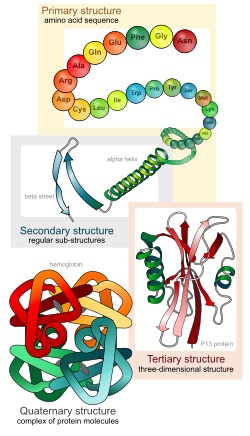
\includegraphics[scale=0.5]{/Users/fran/Documents/Work/tesis/figures/protein_structure_levels_en.png}

	\caption{Hierarchical distribution of layers in protein structure}
	\label{fig:hierarchy_figure}
\end{figure}

\subsection{Protein function}

\par The structure of a protein determines its biological function. However, different \textit{regions} of the structure can perform semi-indepent functions from each other. These regions are referred to as \textbf{protein domains} [REFS!!!!]. A domain is substructure produced by any part of polypedtide chain that can fold independently into a compact and stable structure. Domains on average contain 80-250 residues [REF]. Estimates of the number of domains per protein say that  ~67\% of procaryotik proteins and ~80\% of eukaryotic proteins include more than one domain[REF 259,260 libro protein]. Domains are not only the basic functional units of proteins, but also the evolutionary units of protein evolution [REF]. As proteins have evolved, domains have been modified and combined to build new proteins [REF]. The study of protein domains have became such an important topic in biology  that several databases of protein domains are available. Some of them such as SCOP or CATh are purely based on the structure, while others such as PFAM or INTERPRO include information about the function in their classification. 
\par Domains, and subsequently proteins; perform its biological activity by interacting with other molecules. Proteins can interact with other proteins, constructing a protein-protein complex, with ions or with small-molecules. The substance that is bound to the \textit{target} protein is called the \textbf{ligand}, while the region of the protein where the ligand is binding is called ligand's \textit{binding site}. In the thesis, I will use ligand only for small-molecule compounds while proteins will be considered as equals and will be explicit named as protein-protein interaction[PIE DE NOTA].  The roles played by the ligands are diverse. Table X shows an example of the different functions that a small-molecule ligands can perform in a protein. 

\subsection{Protein-small molecule interaction} \label{ligand_intect}

Binding constants, allosteric and binding-site, induced fit model. Expandir. Imporatante. 

\subsection{Protein modelling}

3D-Structure modelling. 




\subsection{Protein-ligand prediction}


\subsection{Drug discovery}



\begin{table}[h]
  \centering
  \begin{tabular}{|l|l|}
   \hline
    0 & 0 \\ \hline
    0 & 0 \\ \hline    
  \end{tabular}
  \caption{Prova de taula}

\end{table}

\subsection{subsection}
Subsection

\section{Drug discovery}
Second
\subsection{In-silico methods in drug-discovery}
Subsection
\section{Mycobacterium tuberculosis}
\subsection{Tuberculosis treatments and PPcs}
\section{Drug resistance in cancer}
\subsection{Cancer Treatment and drugs}





\chapter{Objectives}
\chapter{nAnnolyze}
\chapter{Predicting targets in MTB}
\chapter{Drug resistance in cancer}



\begin{figure}[b]
  \centering
  
\includegraphics[scale=0.5]{/Users/fran/Documents/Work/tesis/figures/logo_upf.png}
    \caption{Example}
    \label{fig:logo}
\end{figure}





%\bibliography{/Users/fran/Documents/Work/tesis/bibliography/bibliography_tesis}



\backmatter
\printindex

\printbibliography






\end{document}
